\ifx\allfiles\undefined
\documentclass[UTF8, a4paper]{ctexart}

\usepackage{graphicx}
\usepackage{amsmath}
\usepackage{amssymb}
\usepackage{geometry}

\geometry{left=1.0cm, right=1.0cm, top=2.0cm, bottom=1.5cm}
\setlength\parskip{0em}

\graphicspath{{../../valse_webinar/img/}}

\begin{document}
\title{UPSNet: A Unified Panoptic Segmentation Network}
\author{Xiong et al.}
\date{2019.6.24}
\maketitle
\fi
\section{UPSNet: A Unified Panoptic Segmentation Network}

\subsection{Summary} % Summary写完笔记之后最后填,概述文章的内容,以后查阅笔记的时候先看这一段。

本文在Kirillov et al.提出的全景分割模型MR-CNN-PSP\cite{Pano_Seg_Kirillov_2019_CVPR}的基础上进行改进,
提出了一种使用统一的\textbf{backbone}网络同时生成语义分割和实例分割的网络,
并使用\textbf{panoptic head}帮助精确预测每个pixel的class label和instance label,
实现了\textbf{end-to-end}的全景分割。

\subsection{Research Objective} % Research Objective作者的研究目标。

随着CV领域的发展,语义分割和实例分割都已经有很大进展。语义分割侧重基于颜色纹理等信息对于无定形图形进行划分,实例分割侧重于细分每个可数物体。
两者均是处理像素级的视觉场景理解,彼此本应相互促进,但是实际上使用的却是截然不同的处理策略,前者基于FCN,后者基于目标检测得到的bbox。
为了将两者进行互补,提出了全景分割。(类似的任务以前曾经以image parsing, scene parsing 和 holistic scene understanding的名字出现过)

\subsection{Problem} % Problem Statement问题陈述,要解决什么问题?

语义分割和实例分割:
\begin{itemize}
    \item 语义分割无法区分多个同class物体的instance
    \item 实例分割是先进行目标检测然后对bbox中的物体进行分割,无法对背景stuff进行分割
    \item 因此提出全景分割\cite{Pano_Seg_Kirillov_2019_CVPR},同时分割背景stuff和前景thing的instance,使得属于背景stuff的pixel具有类标签,前景thing具有instance label
\end{itemize}

原有全景分割:
\begin{itemize}
    \item 只是简单讲PSPNet的语义分割stuff部分和实例分割的结果进行合并(Heuristics Merging),合并太过粗糙,不能end-to-end训练
    \item 特征提取是分开进行的,计算冗余大
\end{itemize}

\subsection{Method} % Method(s)解决问题的方法/算法是什么?

UPSNet:
\paragraph{backbone} 使用Mask R-CNN\cite{Maskrcnn_He_2017_ICCV}的backbone:ResNet\cite{ResNet_He_2016_CVPR} + FPN\cite{FPN_Lin_2017_CVPR}。
\paragraph{Instance Head} 类Mask R-CNN,有三类输出:bbox回归结果、分类结果、分割mask结果
\paragraph{Segmentation Head} 可变形卷积\cite{Deformable_Conv_Dai_2017_ICCV} + FPN;使用pixel-wise的交叉熵loss
\paragraph{Panoptic Head}
\paragraph{Loss} 8 loss functions: \\
semantic segmentation head (whole image and RoI based pixel-wise classification losses),\\ 
panoptic segmentation head (whole image based pixel-wise classification loss), \\
RPN (box classification, box regression), \\
instance segmentation head (box classification, box regression and mask segmentation).

{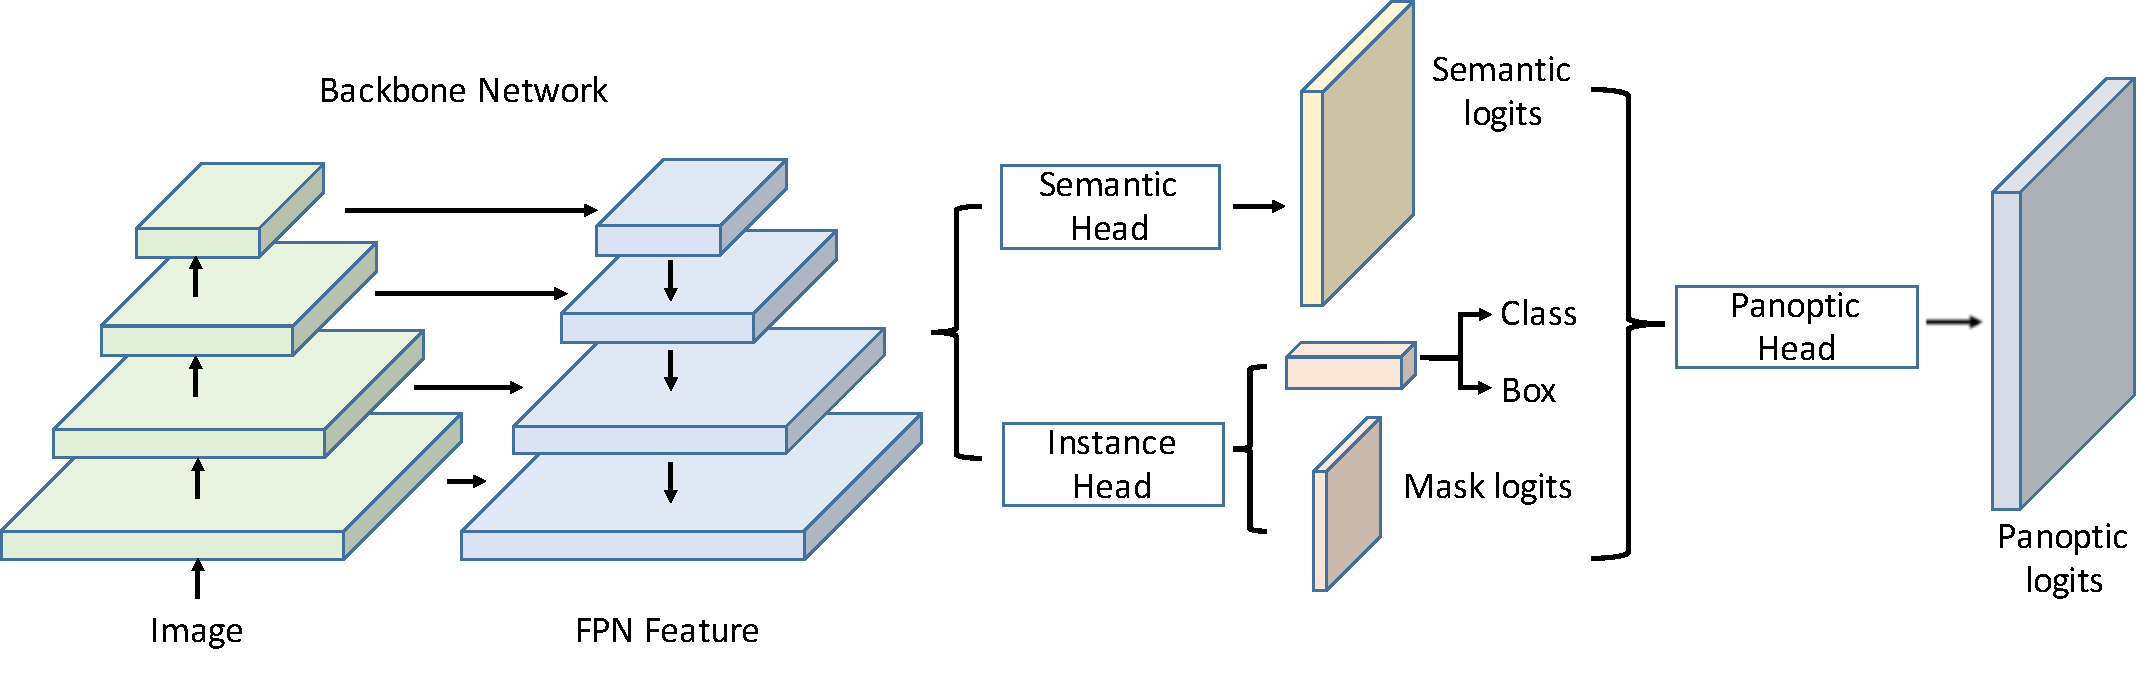
\includegraphics[width=0.95\linewidth]{UPSNet-network}}

\subsection{Evaluation} % Evaluation作者如何评估自己的方法,有没有问题或者可以借鉴的地方。

\paragraph{数据集} MS COCO + Cityscapes + 自制数据集
\paragraph{衡量指标} 分割质量:$PQ = SQ \times RQ$ (total vs. stuff vs. thing)
\begin{equation}
    PQ = {
        \underbrace{\frac{\sum_{(p,g) \in \text{TP}} \text{IoU}(p, g)}{ \vert \text{TP} \vert}}_{\text{SQ}} 
        \underbrace{\frac{\vert \text{TP} \vert}{\vert \text{TP} \vert + \frac{1}{2} \vert \text{FP} \vert + \frac{1}{2} \vert \text{FN} \vert }}_{\text{RQ}}
    } 
\end{equation}

分割速度:Inference time (a single NVIDIA GeForce GTX 1080 Ti GPU and an Intel Xeon E5-2687W CPU (3.00GHz))

\subsection{Conclusion} % Conclusion作者给了哪些strong conclusion, 又给了哪些weak conclusion?

\begin{itemize}
    \item 提出了一种用于全景分割的unified的framework,使用了一个backbone和两个轻量的head实现了同时进行semantic和instance分割,并能够对于unknown类别进行准确预测。
    \item 实验结果表明UPSNet在三个数据集上都达到了SOTA的性能,同时还确保了比其他方法都快。
    \item 将来的work会集中在backbone改进和参数自学习的panoptic head。
\end{itemize}

\subsection{Notes} % Notes在这些框架外额外需要记录的笔记。

超参数设置:\\
使用MSRA的ImageNet预训练模型进行训练,学习率在1500次迭代中从0.002逐步增长到0.02。

图片预处理:\\
COCO数据集训练时中resize到最短边为800,最长边不超过1333,不使用multi-scale训练,进行左右翻转;\\
测试的时候使用multi-scale,最短边resize为$\left\{480; 544; 608; 672; 736; 800; 864; 928; 992; 1056; 1120\right\}$,然后将不同尺寸下的结果进行average。\\
Cityscapes使用了mutil-scale训练,最短边在[800,1024]区间随机resize;\\
测试的时候resize为$\left\{704; 768; 832; 896; 960; 1024; 1088; 1152; 1216; 1280; 1344\right\}$。

\bibliography{../references}
\bibliographystyle{../../IEEEtran}

\ifx\allfiles\undefined
\end{document}
\fi